\section{Задача <<Графический редактор <<Хамелеон>>}

\begin{frame}[t]{Задача <<Графический редактор <<Хамелеон>>}

  \begin{center}
    \LARGE Задача <<Графический редактор <<Хамелеон>>
  \end{center}

  \begin{center}
%    \includegraphics[height=3cm]{}
  \end{center}
\end{frame}

\begin{frame}[t]{Задача <<Графический редактор <<Хамелеон>>}

  \begin{center}
    \LARGE Задача <<Графический редактор <<Хамелеон>>
  \end{center}

  \begin{itemize}
    \item Идея задачи --- Михаил Дворкин
    \item Подготовка тестов --- Павел Кунявский и Никита Иоффе
    \item Визуализатор --- Георгий Корнеев
    \item Разбор задачи --- Павел Кунявский
  \end{itemize}
\end{frame}

\subsection{Формулировка задачи}

\begin{frame}[t]{Формулировка}
  \begin{itemize}
    \item Задано квадратное поле, которое требуется покрасить по данной картинке.
    \item Можно перемещаться в четырёх направлениях.
    \item При перемещении можно либо перекрасить клетку в цвет хамелеона, либо хамелеона в цвет клетки.
  \end{itemize}
  Результат:
  \begin{itemize}
    \item Последовательность ходов, приводящая к необходимой покраске.
  \end{itemize}
\end{frame}

\subsection{Структура тестов}

\begin{frame}[t]{Структура тестов}
    \begin{itemize}
        \item Первый тест --- черный квадрат.
        \begin{itemize}
            \item Обойти квадрат как угодно
        \end{itemize}

        
\includegraphics[height=4cm]{cham01.png}
    \end{itemize}
\end{frame}
\begin{frame}[t]{Структура тестов}
    \begin{itemize}
        \item Следующие 4 теста --- связные области
        \begin{itemize}
            \item Обойти область в глубину
        \end{itemize}
    \end{itemize}
    \vspace{-1em}
    \begin{center}
        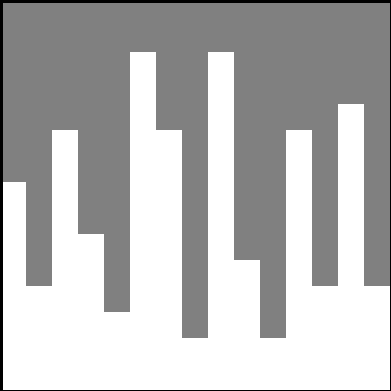
\includegraphics[height=2.8cm]{cham02.png}
        \quad
        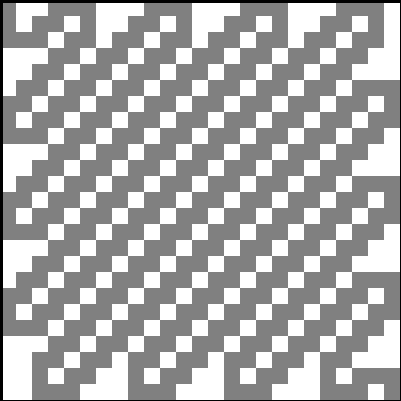
\includegraphics[height=2.8cm]{cham03.png}
        \\
        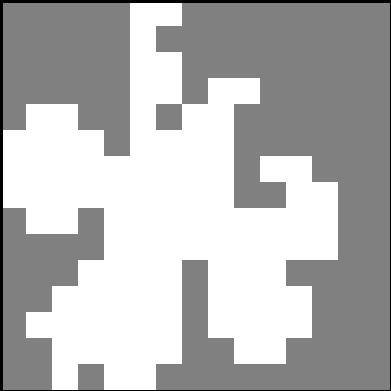
\includegraphics[height=2.8cm]{cham04.png}
        \quad
        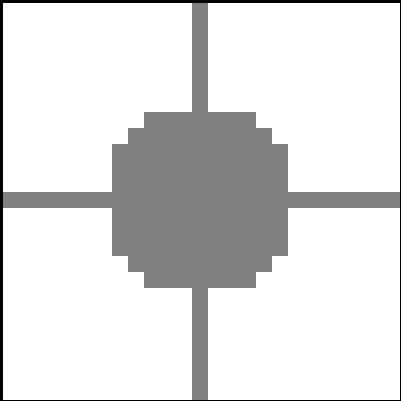
\includegraphics[height=2.8cm]{cham05.png}
    \end{center}
\end{frame}
\begin{frame}[t]{Структура тестов}
    \begin{itemize}
        \item Следующие 3 теста --- конструкции %, для которых можно придумать специальное решение
        \begin{itemize}
            \item Можно написать специальное решение
        \end{itemize}
    \end{itemize}
    \begin{center}
        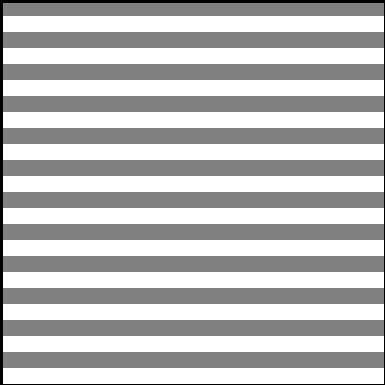
\includegraphics[height=3cm]{cham06.png}
        \quad
        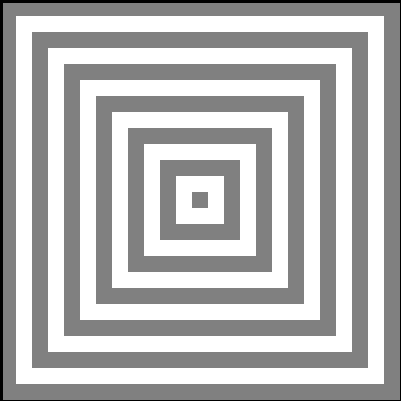
\includegraphics[height=3cm]{cham07.png}
        \quad
        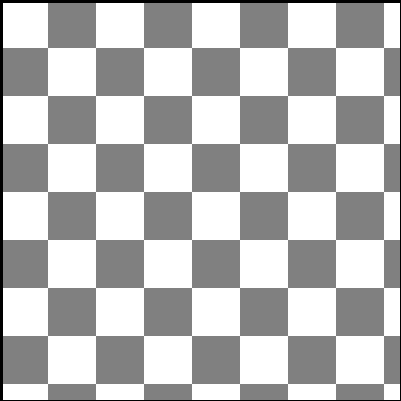
\includegraphics[height=3cm]{cham08.png}
    \end{center}
\end{frame}
\begin{frame}[t]{Структура тестов}
        Остальные тесты решаются общим методом

        \begin{center}
        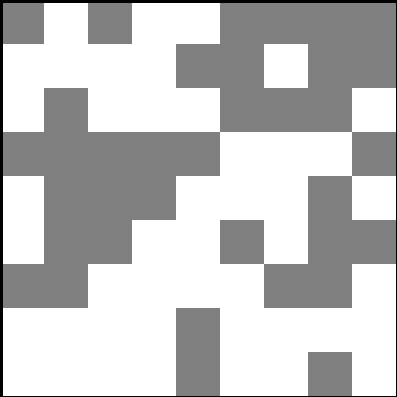
\includegraphics[height=3cm]{cham09.png}
        ~
        
\includegraphics[height=3cm]{cham10.png}
        ~
        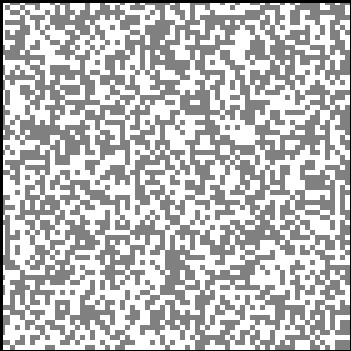
\includegraphics[height=3cm]{cham11.png}
        \par
        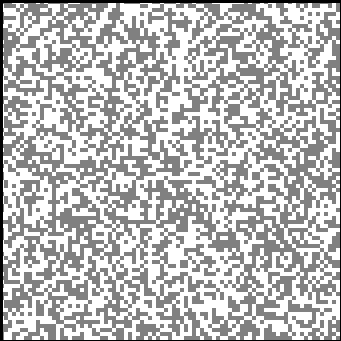
\includegraphics[height=3cm]{cham12.png}
        ~
        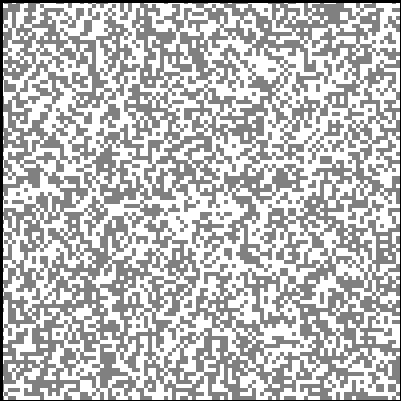
\includegraphics[height=3cm]{cham13.png}
        ~
        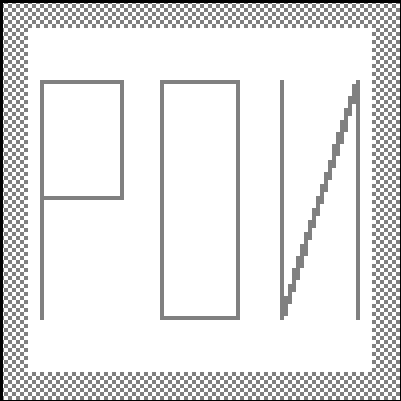
\includegraphics[height=3cm]{cham14.png}
        \end{center}
\end{frame}
\begin{frame}[t]{Структура тестов}
        Остальные тесты решаются общим методом

        \begin{center}
        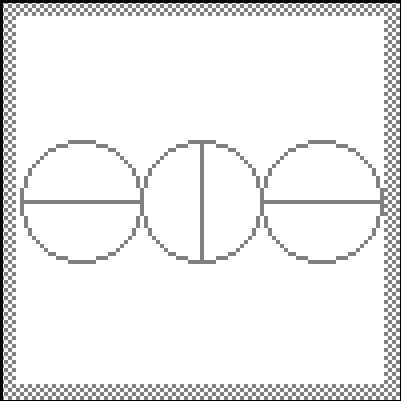
\includegraphics[height=3cm]{cham15.png}
        ~
        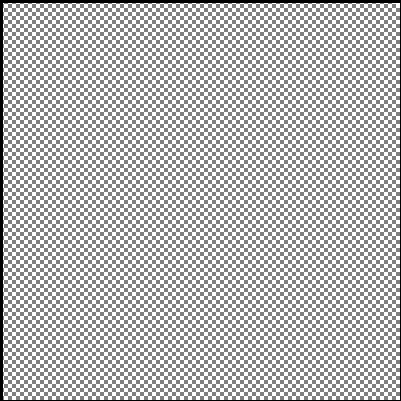
\includegraphics[height=3cm]{cham16.png}
        ~
        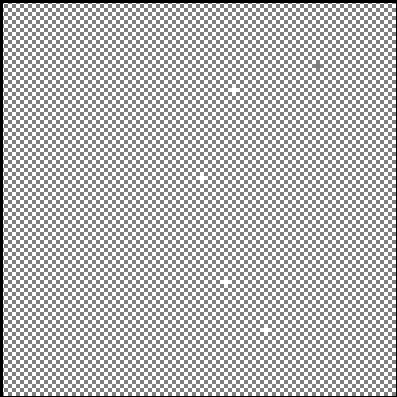
\includegraphics[height=3cm]{cham17.png}
        \par
        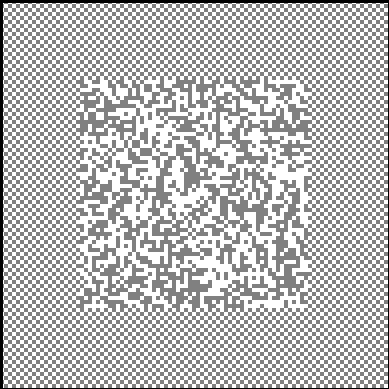
\includegraphics[height=3cm]{cham18.png}
        ~
        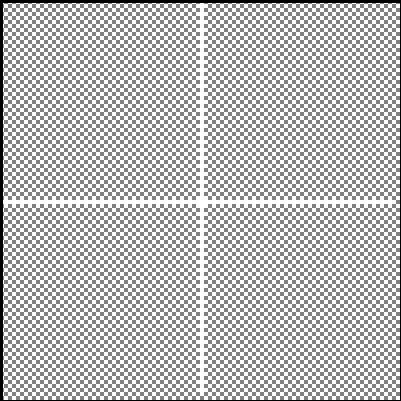
\includegraphics[height=3cm]{cham19.png}
        ~
        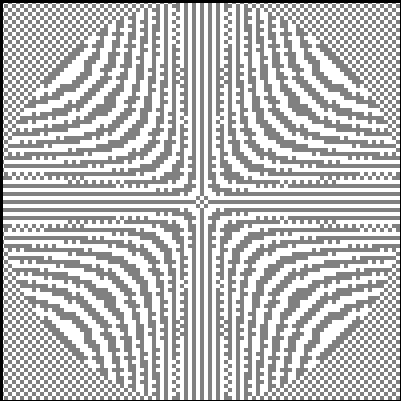
\includegraphics[height=3cm]{cham20.png}
        \end{center}
\end{frame}


\subsection{Решение}

\begin{frame}[t]{Решение}
  \begin{itemize}
%   \item В тестах можно заметить большое количество частей, покрашенных в шахматном порядке.
    \item Докажем, что покрасить шахматную доску нельзя
  \end{itemize}
  \begin{itemize}
    \item Для этого посмотрим на последнее перекрашивание. Оно создает две клетки одинакого цвета рядом.
    \item Значит, в любой покраске такие есть, а в шахматной нет.
  \end{itemize}
%  \end{itemize}
\end{frame}

\begin{frame}[t]{Решение}
  \begin{itemize}
    \item Докажем, что всё остальное покрасить можно.
  \end{itemize}
  \begin{itemize}
    \item Выберем две соседние клетки, которые должны быть покрашены в одинаковый цвет. Назовем выбранную пару клеток {\it базой}.
    \item Покрасим две клетки базы в разные цвета.
    \item Для определенности будем считать базу горизонтальной, второй случай симметричен.
  \end{itemize}
\end{frame}

\begin{frame}[t]{Решение}
  \begin{itemize}
    \item Будем красить доску отдельно снизу от базы, отдельно сверху. Рассмотрим нижнюю часть.
    \item Будем красить строки снизу вверх. Строку красим отдельно слева от базы,
    отдельно справа.
    \item Обе части будем красить от края к базе.
    \item Чтобы покрасить клетку, надо переместиться на базу в клетку с нужным цветом
        и вернуться, перекрашивая.
  \end{itemize}
\end{frame}

\begin{frame}[t]{Решение}
  \begin{itemize}
    \item Таким образом получится покрасить всё, кроме части вокруг базы.
    \item Её можно разобрать руками. Для этого может понадобиться испортить базу.
    \item Таким образом получено решение, делающее $N^3$ ходов.
  \end{itemize}
\end{frame}

\begin{frame}[t]{Решение}
  \begin{itemize}
    \item Для того, чтобы получить квадратичное решение, надо не ходить на базу для каждой клетки.
    \item Например для этого можно покрасить все чётные строки в один цвет, а все нечётные "--- в другой за один проход по полю.
  \end{itemize}
\end{frame}

\begin{frame}[t]{Решение}
  \begin{itemize}
    \item После этого можно разносить цвет, проходя на строку ближе к базе и перенося другой цвет на очередную строку.
    \item При этом не получится покрасить последнюю строку, но её можно покрасить старым алгоритмом за квадрат.
  \end{itemize}
\end{frame}

\subsection{Оптимизации}

\begin{frame}[t]{Оптимизации}
    \begin{itemize}
        \item Такое решение уже должно укладываться в $5\cdot N^2$ ходов.
        \item Строки вокруг базы можно покрасить аналогично, проходя по столбцам.
    \end{itemize}
\end{frame}

\begin{frame}[t]{Оптимизации}
    \begin{itemize}
        \item Такой алгоритм уже занимает $\frac{1}{2} \cdot N^2$ ходов на покраску клеток через строку. При проходе назад
            мы тратим еще ходов не более $3 \cdot N^2$.
        \item Применим такую оптимизацию: если несколько подряд клеток не того цвета, будем красить их за один проход.
            Тогда мы будем тратить три хода на не более чем половину клеток. Это уменьшит длину решения на $N^2$ ходов.
    \end{itemize}
\end{frame}

\begin{frame}[t]{Оптимизации}
    \begin{itemize}
        \item Тогда решение займет $2.5 \cdot N^2$ ходов. Неучтённые линейные части занимают меньше $\frac{1}{2} \cdot N^2$.
    \end{itemize}
\end{frame}


\begin{frame}
  \begin{center}
    {\LARGE Вопросы?}
  \end{center}
\end{frame}
